\documentclass[border=12pt]{standalone}
\def\pgfsysdriver{pgfsys-dvisvgm.def}
\usepackage[dvisvgm]{xcolor}
\usepackage{xeCJK}
\setCJKmainfont{HaranoAjiGothic-Regular.otf}[BoldFont=HaranoAjiGothic-Bold.otf]
\setCJKsansfont{HaranoAjiGothic-Regular.otf}[BoldFont=HaranoAjiGothic-Bold.otf]
\usepackage{amsmath,amssymb,tikz,lmodern}
\usetikzlibrary{arrows.meta,positioning,calc,fit,backgrounds}
\renewcommand{\familydefault}{\sfdefault}
\definecolor{ink}{HTML}{25322F}
\definecolor{green}{HTML}{246657}
\definecolor{tint}{HTML}{EEF4F0}
\definecolor{soft}{HTML}{C6D2CC}
\definecolor{muted}{HTML}{52615B}
\newif\ifJapanese
\newcommand{\Tx}[2]{\ifJapanese #1\else #2\fi}
\newcommand{\Eff}{\overline{\operatorname{Eff}}}
\newcommand{\heading}[3]{{\color{green}\bfseries #1\quad\Tx{#2}{#3}}\\[5pt]}
% A white rectangle makes the complete citation label clickable, including spaces.
\newcommand{\refurl}[2]{\special{dvisvgm:raw <a xlink:href="#1" target="_blank" rel="noopener noreferrer">}{\setlength{\fboxsep}{0pt}\colorbox{white}{\color{green}\underline{\strut #2}}}\special{dvisvgm:raw </a>}}
\newcommand{\refedge}[3]{\refurl{\csname source#1\endcsname\string##page=#2}{#3}}
\newcommand{\SF}[2]{\refedge{sf}{#1}{#2}}
% GitHub's file preview does not support PDF page fragments.
\newcommand{\LA}[2]{\refurl{\sourcela}{#2}}
\newcommand{\Sch}[2]{\refedge{sch}{#1}{#2}}
\newcommand{\PS}[2]{\refedge{ps}{#1}{#2}}
\tikzset{
 card/.style={draw=soft,fill=white,rounded corners=2pt,align=left,text=ink,font=\fontsize{10.5}{14}\selectfont,inner xsep=12pt,inner ysep=10pt,text width=14.4cm},
 half/.style={card,text width=6.45cm,minimum height=2.05cm},
 result/.style={card,draw=green,fill=tint,line width=.9pt},
 reason/.style={align=left,text=muted,font=\fontsize{9}{12}\selectfont,inner sep=0pt,text width=12.7cm},
 branchreason/.style={reason,text width=5.95cm},
 edge/.style={-{Stealth[length=2.4mm]},draw=green,line width=1pt},
 wire/.style={draw=green,line width=1pt},
}
% Keep the arrow in a dedicated left gutter; explanations never cover it.
\newcommand{\flow}[3]{
 \coordinate (#2-from) at ($(#1.south)+(-6.9,0)$);
 \coordinate (#2-to) at ($(#2.north)+(-6.9,0)$);
 \draw[edge] (#2-from)--(#2-to);
 \node[reason,anchor=west] (#2-reason) at ($(#2-from)!.5!(#2-to)+(.55,0)$) {#3};
}


\newcommand{\CiteSource}[2]{\refurl{\csname source#1\endcsname}{#2}}

\expandafter\def\csname sourceS\endcsname{https://github.com/openai/math/blob/adc7f1241b42e322a6451854ab7e4b4c146bf78a/preprints/Lifting-sections-from-the-reduced-support-of-an-adjoint-September-27-2026/paper.pdf}
\expandafter\def\csname sourceNV\endcsname{https://github.com/openai/math/blob/adc7f1241b42e322a6451854ab7e4b4c146bf78a/preprints/Fourfold-nonvanishing-by-minimal-metrics-and-moving-jets-September-27-2026/paper.pdf}
\expandafter\def\csname sourceFG\endcsname{https://www.math.kyoto-u.ac.jp/~fujino/fg-comp-final.pdf}
\expandafter\def\csname sourceKS\endcsname{https://people.math.harvard.edu/~mpopa/papers/oxford.pdf}
\expandafter\def\csname sourceHash\endcsname{https://arxiv.org/html/1609.00121v4}
\expandafter\def\csname sourceBir\endcsname{https://arxiv.org/pdf/0706.1792}
\expandafter\def\csname sourceSaito\endcsname{https://doi.org/10.2977/PRIMS/1195171082}
\expandafter\def\csname sourceUfour\endcsname{https://github.com/openai/math/blob/adc7f1241b42e322a6451854ab7e4b4c146bf78a/preprints/Uniform-effective-log-Iitaka-fibrations-for-fourfolds-September-26-2026/paper.pdf}

\Japanesefalse
\begin{document}
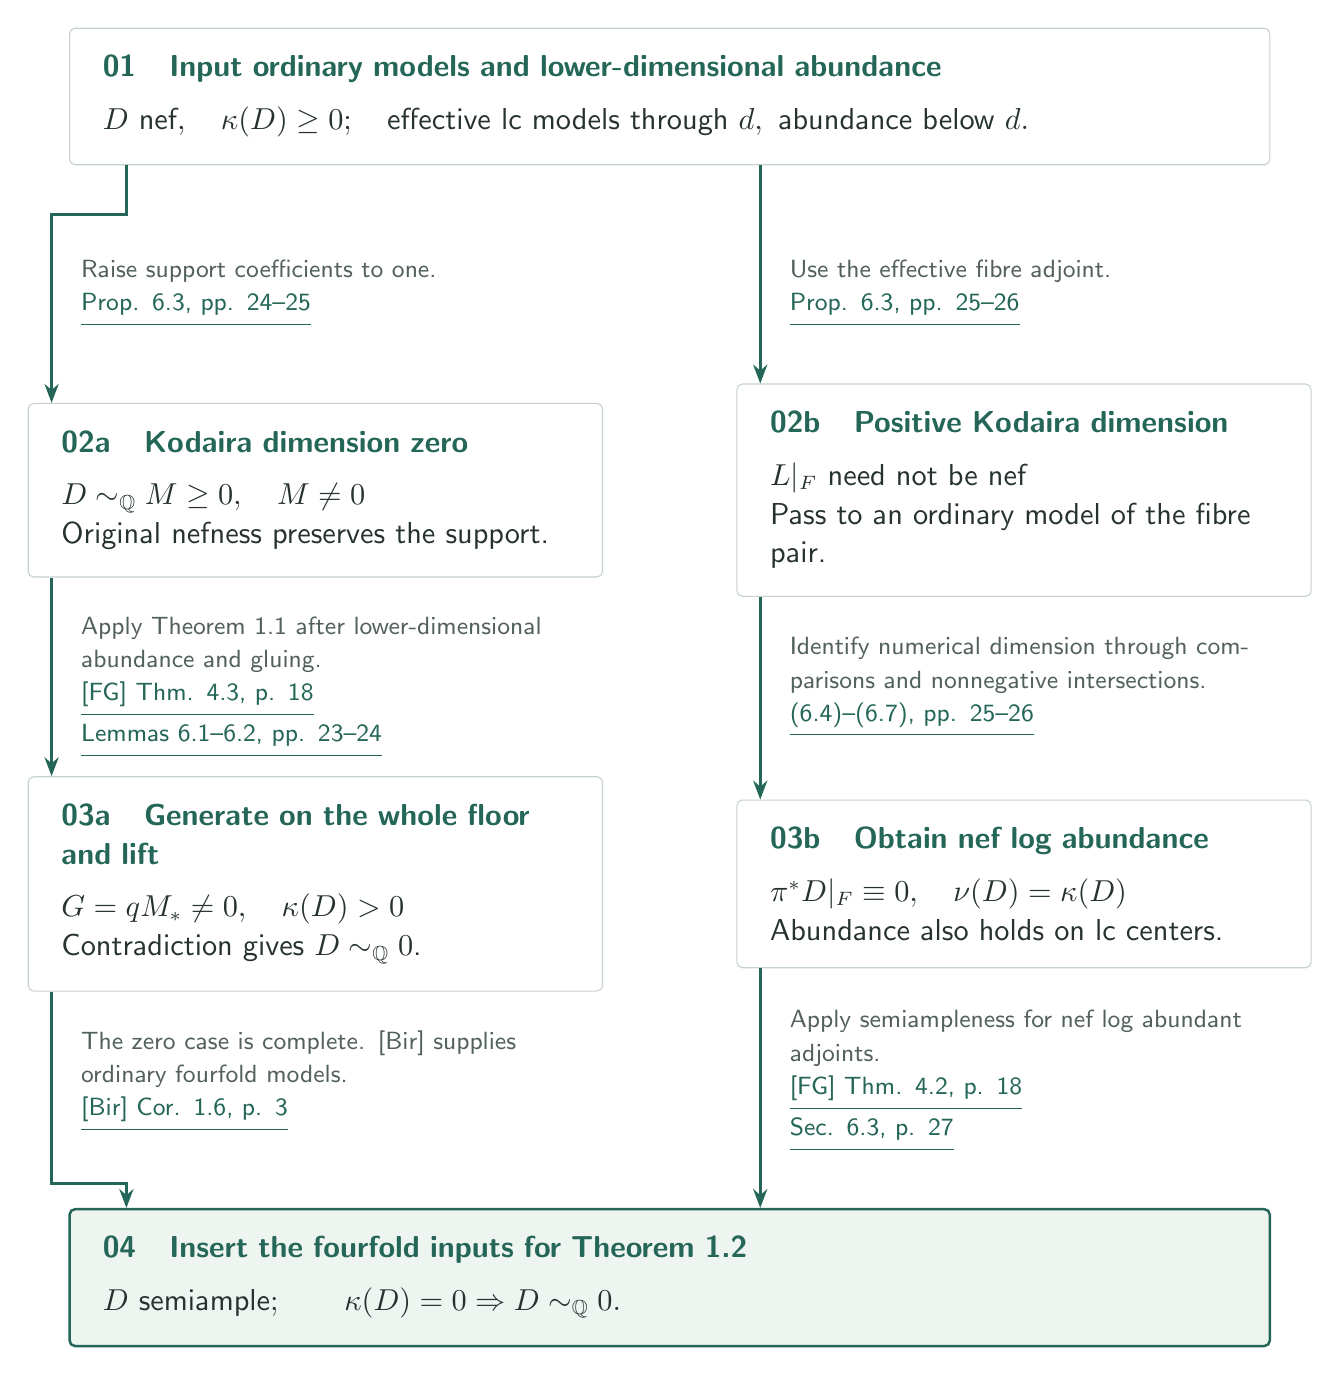
\begin{tikzpicture}
\node[card] (start) at (0,0) {\heading{01}{通常のモデルと低次元 abundance を入力する}{Input ordinary models and lower-dimensional abundance}$D\ \text{nef},\quad\kappa(D)\ge0;\quad\text{effective lc models through }d,\ \text{abundance below }d.$};
\node[half] (zero) at (-4.5,-5) {\heading{02a}{小平次元0}{Kodaira dimension zero}$D\sim_{\mathbb Q}M\ge0,\quad M\ne0$\\\Tx{元の nef 性で台を残す。}{Original nefness preserves the support.}};
\node[half] (pos) at (4.5,-5) {\heading{02b}{正の小平次元}{Positive Kodaira dimension}$L|_F\ \text{need not be nef}$\\\Tx{ファイバー対の通常のモデルへ移る。}{Pass to an ordinary model of the fibre pair.}};
\node[half] (zout) at (-4.5,-10) {\heading{03a}{全 floor で生成して持ち上げる}{Generate on the whole floor and lift}$G=qM_*\ne0,\quad\kappa(D)>0$\\\Tx{矛盾より $D\sim_{\mathbb Q}0$。}{Contradiction gives $D\sim_{\mathbb Q}0$.}};
\node[half] (pout) at (4.5,-10) {\heading{03b}{nef log abundance を得る}{Obtain nef log abundance}$\pi^*D|_F\equiv0,\quad\nu(D)=\kappa(D)$\\\Tx{lc center にも abundance。}{Abundance also holds on lc centers.}};
\node[result] (out) at (0,-15) {\heading{04}{四次元の入力で Theorem 1.2 を得る}{Insert the fourfold inputs for Theorem 1.2}$D\ \text{semiample};\qquad\kappa(D)=0\Rightarrow D\sim_{\mathbb Q}0.$};
\draw[edge] ($(start.south)+(-6.9,0)$)--(-6.9,-1.5)--(-7.85,-1.5)--($(zero.north)+(-3.35,0)$);
\draw[edge] ($(start.south)+(1.15,0)$)--($(pos.north)+(-3.35,0)$);
\node[branchreason] at (-4.5,-2.5) {\Tx{有効代表元の台を係数1へ上げる。}{Raise support coefficients to one.}\\\CiteSource{S}{Prop. 6.3, pp. 24--25}};
\node[branchreason] at (4.5,-2.5) {\Tx{飯高ファイバーの有効随伴因子を使う。}{Use the effective fibre adjoint.}\\\CiteSource{S}{Prop. 6.3, pp. 25--26}};
\draw[edge] ($(zero.south)+(-3.35,0)$)--($(zout.north)+(-3.35,0)$);
\draw[edge] ($(pos.south)+(-3.35,0)$)--($(pout.north)+(-3.35,0)$);
\node[branchreason] at (-4.5,-7.5) {\Tx{低次元 abundance と gluing の後、Theorem 1.1 を適用。}{Apply Theorem 1.1 after lower-dimensional abundance and gluing.}\\\CiteSource{FG}{[FG] Thm. 4.3, p. 18}\\\CiteSource{S}{Lemmas 6.1--6.2, pp. 23--24}};
\node[branchreason] at (4.5,-7.5) {\Tx{比較式と非負交点数から数値次元を同定。}{Identify numerical dimension through comparisons and nonnegative intersections.}\\\CiteSource{S}{(6.4)--(6.7), pp. 25--26}};
\draw[edge] ($(zout.south)+(-3.35,0)$)--(-7.85,-13.8)--(-6.9,-13.8)--($(out.north)+(-6.9,0)$);
\draw[edge] ($(pout.south)+(-3.35,0)$)--($(out.north)+(1.15,0)$);
\node[branchreason] at (-4.5,-12.5) {\Tx{零の場合は既に終了。四次元の通常のモデルは [Bir] が供給。}{The zero case is complete. [Bir] supplies ordinary fourfold models.}\\\CiteSource{Bir}{[Bir] Cor. 1.6, p. 3}};
\node[branchreason] at (4.5,-12.5) {\Tx{nef log abundant 随伴因子に適用。}{Apply semiampleness for nef log abundant adjoints.}\\\CiteSource{FG}{[FG] Thm. 4.2, p. 18}\\\CiteSource{S}{Sec. 6.3, p. 27}};
\end{tikzpicture}
\end{document}
